% ==============================================================================
% SECCIÓN DE VISIÓN COMPUTACIONAL Y OCR (FORMATO IEEEtran)
% ==============================================================================

\section{Pipeline de Visi\'on por Computador y Reconocimiento de Caracteres}
\label{sec:vision_pipeline}

El pipeline sensorial transforma im\'agenes sin procesar (fotograf\'{\i}as m\'oviles con sombras y perspectiva o capturas digitales) en una representaci\'on simb\'olica estructurada. Como se esquematiza en la Fig.~\ref{fig:vision_stages}, el procesamiento se divide en: rectificaci\'on geom\'etrica, inferencia topol\'ogica de la grilla, segmentaci\'on morfol\'ogica de glifos y clasificaci\'on probabil\'{\i}stica mediante una red neuronal convolucional adaptada v\'{\i}a \textit{Fine-Tuning}.

\begin{figure*}[t]
\centering
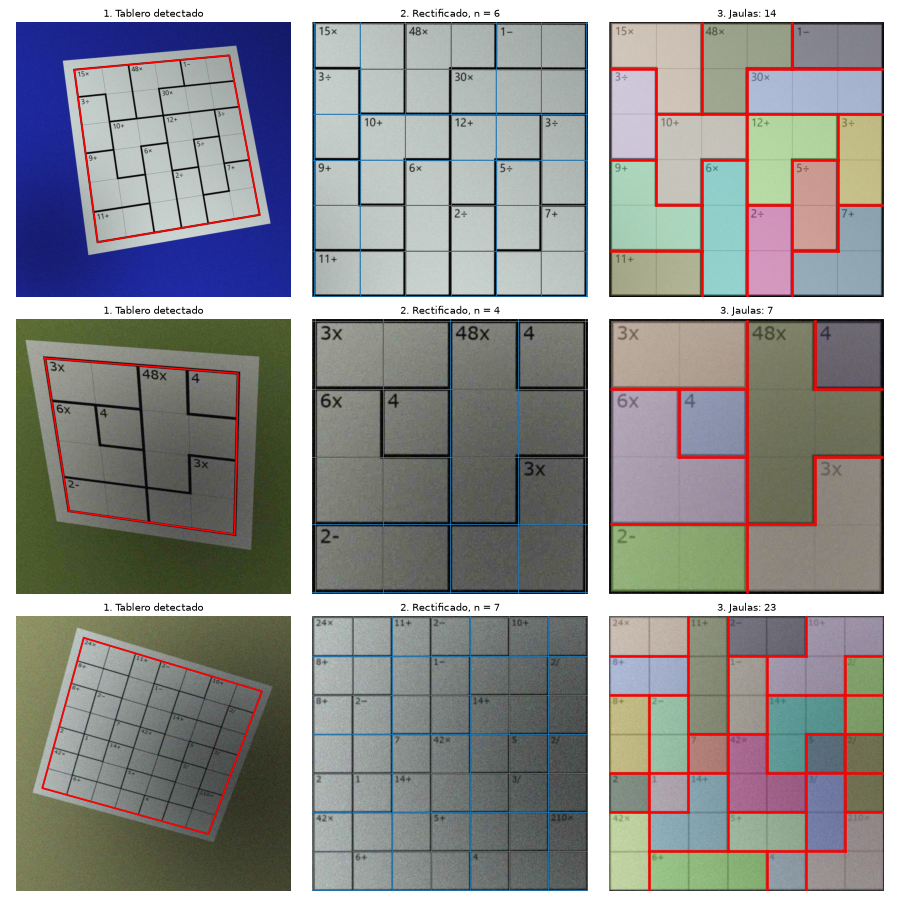
\includegraphics[width=0.95\textwidth]{figs/vision_stages.png}
\caption{Etapas del pipeline de visi\'on computacional: (a) Imagen de entrada con perspectiva y sombras, (b) Binarizaci\'on adaptativa y detecci\'on cuadrangular, (c) Rectificaci\'on proyectiva homogr\'afica $H$, (d) Extracci\'on de l\'{\i}neas y clasificaci\'on de bordes de jaula, (e) Agrupaci\'on conexa por \textit{Union-Find}, y (f) Reconocimiento OCR de etiquetas aritm\'eticas.}
\label{fig:vision_stages}
\end{figure*}

\subsection{Rectificaci\'on Geom\'etrica y Detecci\'on Estructural}
El contorno dominante del tablero se localiza aproximando pol\'{\i}gonos convexos cuadrangulares sobre la imagen binarizada. Para anular la distorsi\'on de perspectiva, se calcula la matriz homogr\'afica proyectiva $H \in \mathbb{R}^{3 \times 3}$~\cite{bradski2000opencv} mapeando las cuatro esquinas hacia un lienzo frontal normalizado de dimensi\'on can\'onica $W \times H$:
\begin{equation}
    \begin{bmatrix} x' \\ y' \\ 1 \end{bmatrix} \sim H \begin{bmatrix} x \\ y \\ 1 \end{bmatrix}
\end{equation}

La inferencia del orden $n \in [3, 9]$ se ejecuta mediante perfiles de proyecci\'on de gradientes morfol\'ogicos verticales y horizontales, identificando la periodicidad espacial de las crestas divisorias.

La separaci\'on entre l\'{\i}neas internas delgadas y bordes gruesos delimitadores de jaula (\textit{cages}) se modela mediante el algoritmo de Otsu~\cite{otsu1979threshold} aplicado sobre los perfiles de intensidad unidimensionales a lo largo de cada frontera entre celdas. Con la matriz de adyacencia de fronteras, se agrupan las celdas conexas pertenecientes a la misma jaula mediante la estructura de datos \textit{Union-Find} con compresi\'on de caminos~\cite{tarjan1975efficiency}, garantizando una complejidad casi lineal $\mathcal{O}(n^2 \alpha(n^2))$.

\subsection{Mejoras Robustas de Preprocesamiento y Segmentaci\'on}
Durante las evaluaciones con degradaci\'on f\'{\i}sica severa, se incorporaron cuatro mecanismos de robustez:
\begin{enumerate}
    \item \textbf{Supresi\'on Perif\'erica de Cuadr\'{\i}cula:} Residuos de las l\'{\i}neas lim\'{\i}trofes de celda distorsionaban el c\'alculo de la altura de referencia tipogr\'afica $h_{\text{ref}}$. La rutina \texttt{clean\_border\_lines} descarta componentes con elongaci\'on vertical ($h \ge 0.35 \cdot h_{\text{celda}}$, $w \le 3\text{ px}$) u horizontal en los bordes marginales ($x \le 2$ o $x \ge w-4$).
    \item \textbf{Binarizaci\'on Adaptativa ante Sombras Locales:} El umbral global de Otsu colapsaba en regiones de iluminaci\'on heterog\'enea cuando la fracci\'on de tinta superaba el 18\%. El sistema conmuta din\'amicamente a una normalizaci\'on de fondo por desenfoque gaussiano de baja frecuencia:
    \begin{equation}
        I_{\text{norm}} = \text{clip}\left(\frac{I}{\mathcal{G}_{\sigma=31}(I)} \times 255, \; 0, \; 255\right)
    \end{equation}
    restituyendo el contraste de glifos en gradientes lum\'{\i}nicos pronunciados.
    \item \textbf{Hip\'otesis Combinadas de Segundo Orden:} En jaulas con n\'umeros de dos d\'{\i}gitos (e.g., $14+$, $48\times$), la proyecci\'on vertical puede fusionar glifos debido al \textit{kerning} estrecho. Se eval\'uan combinaciones m\'ultiples de cortes verticales ponderadas log-probabil\'{\i}sticamente.
    \item \textbf{Poda Sint\'actica Can\'onica a Priori:} Seg\'un las reglas formales de KenKen, los operadores de resta ($-$) y divisi\'on ($\div$) son operaciones binarias no asociativas y est\'an estrictamente restringidas a jaulas de $|V_c| = 2$. Toda hip\'otesis sensorial que asigne $-$ o $\div$ a jaulas de $|V_c| \ge 3$ es podada de forma inmediata, evitando que ruido sensorial introduzca candidatos matem\'aticamente inadmisibles.
\end{enumerate}

\subsection{Clasificador GlyphCNN y Estrategia de Fine-Tuning}
Para el reconocimiento \'optico de caracteres se implement\'o la red convolucional especializada \texttt{GlyphCNN}.

\subsubsection{Arquitectura}
La red procesa recortes normalizados de $32 \times 32$ p\'{\i}xeles en escala de grises. Posee tres bloques convolucionales con normalizaci\'on por lotes (\textit{BatchNorm2D}), activaci\'on ReLU y \textit{MaxPool2D} (filtros 32, 64 y 64), seguidos de \textit{Dropout} ($p=0.25$) y dos capas densas ($512 \to 14$), totalizando $\approx 403{,}000$ par\'ametros entrenables y 14 clases (d\'{\i}gitos $\{0, \dots, 9\}$ y operadores $\{+, -, \times, \div\}$).

\subsubsection{Fine-Tuning con Hard Example Mining y Focal Loss}
Para maximizar la precisi\'on sobre glifos degradados sin alterar la representaci\'on general del modelo base (\texttt{models/ocr\_cnn.pt}, preservado intacto con SHA-256 verificado), se entren\'o una variante especializada (\texttt{models/ocr\_cnn\_finetuned.pt}) mediante:
\begin{itemize}
    \item \textbf{Corpus Focalizado:} 33{,}122 glifos balanceados mediante miner\'{\i}a de ejemplos dif\'{\i}ciles (31{,}093 sint\'eticos con perturbaciones morfol\'ogicas de trazo $x^\gamma$ con $\gamma \in [0.75, 1.35]$, ruido impulsivo y rotaci\'on continua $\pm 10^\circ$; y 2{,}029 glifos recortados de tableros reales degradados).
    \item \textbf{MultiClass Focal Loss:} Formulada con modulaci\'on de clases ambiguas y \textit{Label Smoothing} ($\epsilon = 0.02$)~\cite{lin2017focal}:
    \begin{equation}
        \text{FL}(p_t) = -\alpha_t (1 - p_t)^\gamma \log(p_t)
    \end{equation}
    con $\gamma = 1.5$ y ponderaciones: $\alpha_{\div} = 1.40$, $\alpha_{+} = 1.35$, $\alpha_{-} = 1.25$, $\alpha_{\times} = 1.25$ y $\alpha_{\text{d\'{\i}gitos}} = 1.00$.
    \item \textbf{Congelamiento Selectivo (\textit{Layer Freezing}):} En las \'epocas 1 y 2 se congelaron los filtros de bajo nivel (Bloque 1), adaptando las capas densas con $lr = 2 \times 10^{-4}$. En las \'epocas 3 a 8 se descongel\'o la totalidad de la red con planificador \textit{Cosine Annealing} descendiendo hasta $10^{-5}$.
\end{itemize}

\begin{figure}[htbp]
\centering
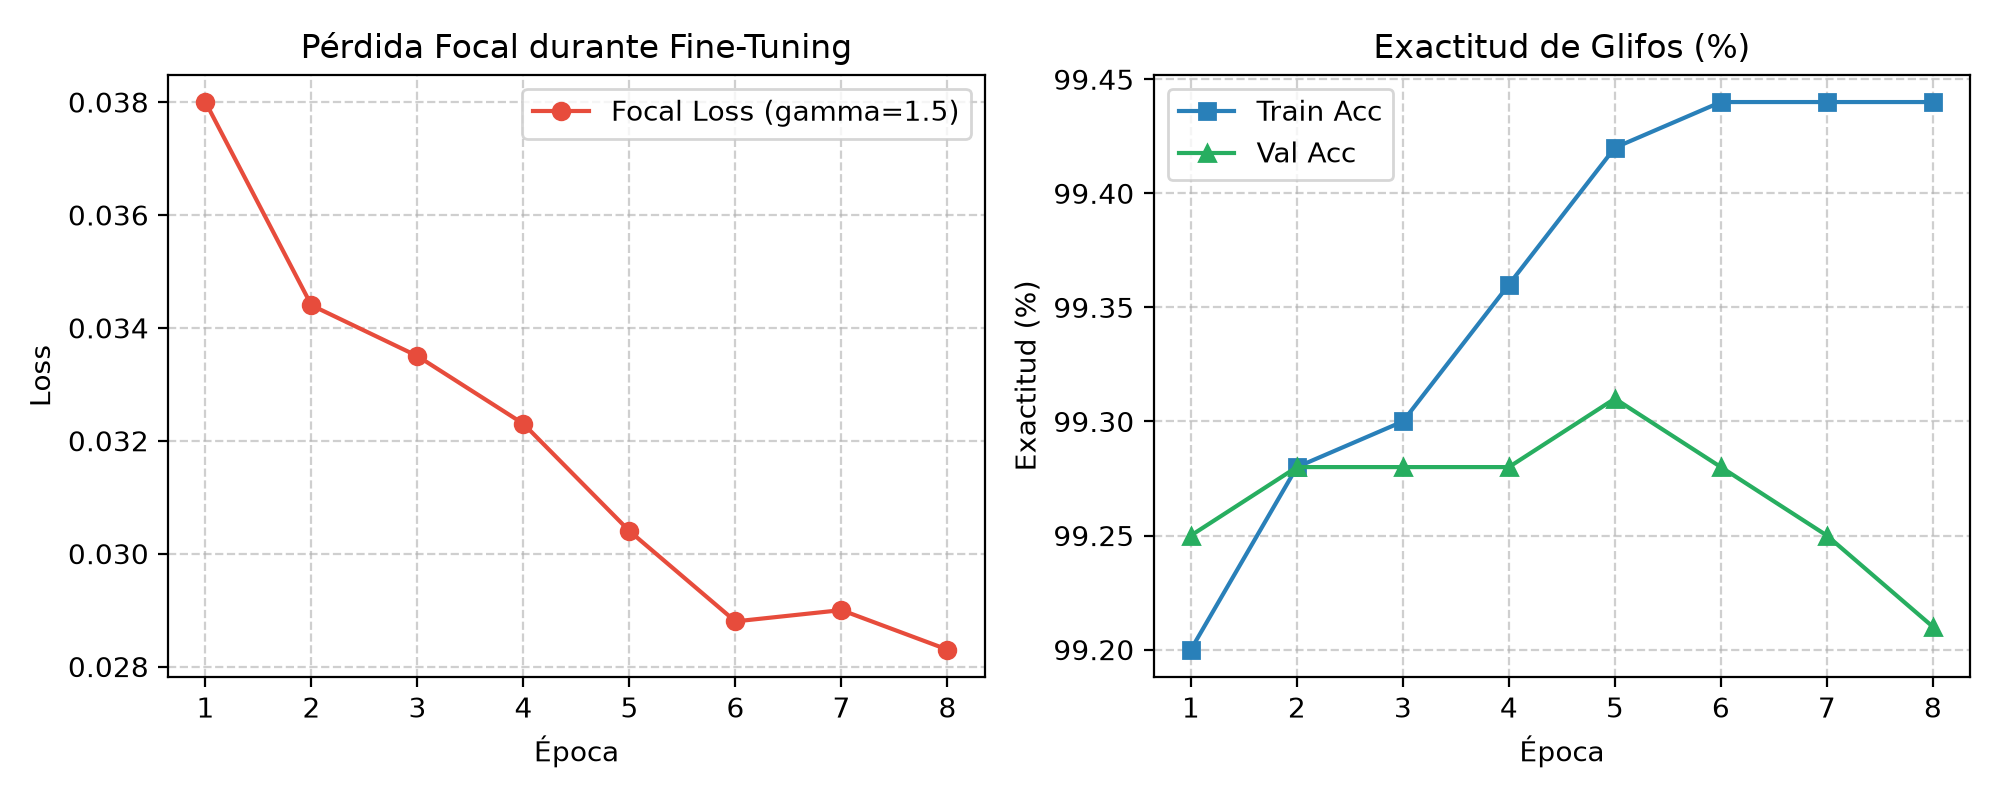
\includegraphics[width=\linewidth]{figs/cnn_finetuning_curves.png}
\caption{Curvas de convergencia del proceso de Fine-Tuning de \texttt{GlyphCNN}: evoluci\'on de la p\'erdida Focal Loss multiclase y exactitud de validaci\'on a lo largo de las 8 \'epocas de entrenamiento.}
\label{fig:cnn_curves}
\end{figure}

Como ilustra la Fig.~\ref{fig:cnn_curves}, el mejor punto de control se consolid\'o en la \'epoca 5 con una exactitud de validaci\'on del $99.31\%$ y p\'erdida de $0.0304$.

\subsection{Evaluaci\'on Experimental y M\'etricas de Error}
El rendimiento del sistema de visi\'on se evalu\'o cuantitativamente en tres entornos:
\begin{enumerate}
    \item \textbf{Synthetic Normal (300 im\'agenes, 12{,}266 glifos):} Tableros bajo iluminaci\'on homog\'enea.
    \item \textbf{Synthetic Hard (150 im\'agenes, 4{,}859 glifos):} Sombras no uniformes, vi\~neteado y ruido de sensor.
    \item \textbf{Challenge Stress (50 im\'agenes, 1{,}778 glifos):} Tableros filtrados donde la lectura Top-1 presenta al menos una inconsistencia o fallo sensorial.
\end{enumerate}

\subsubsection{Comparativa General por Nivel de Entidad}
En el Cuadro~\ref{tab:global_metrics} se contrastan las m\'etricas de reconocimiento por glifo individual, por jaula completa (Top-1 y Top-$k$), y por tablero integral. Mientras que la exactitud por glifo individual en el dataset normal alcanza el $99.51\%$, la exactitud por tablero completo sin asistencia del solver es del $82.00\%$. La integraci\'on de candidatos Top-$k$ junto al motor de CP eleva la tasa de tableros resueltos al récord del \textbf{90.33\%} (271 de 300 tableros).

\begin{table}[htbp]
\caption{M\'etricas de Percepci\'on por Nivel de Entidad y Dataset}
\label{tab:global_metrics}
\centering
\footnotesize
\setlength{\tabcolsep}{3.0pt}
\begin{tabular}{@{}lccc@{}}
\toprule
\textbf{M\'etrica Evaluada} & \textbf{Normal} & \textbf{Hard} & \textbf{Stress} \\
\midrule
Im\'agenes Evaluadas & 300 & 150 & 50 \\
Glifos Analizados & 12{,}266 & 4{,}859 & 1{,}778 \\
Exactitud por Glifo & \textbf{99.51\%} & \textbf{90.99\%} & \textbf{89.43\%} \\
Segmentaci\'on de Jaula OK & 96.50\% & 75.80\% & 80.50\% \\
Jaula Top-1 Exacta & 97.50\% & 74.30\% & 83.80\% \\
Jaula Top-$k$ (con alternativas) & \textbf{99.20\%} & \textbf{84.40\%} & \textbf{93.90\%} \\
Tablero Directo (sin CP) & 82.00\% & 32.00\% & 4.00\% \\
Tablero Resuelto (Top-$k$ + CP) & \textbf{90.33\%} & \textbf{44.67\%} & \textbf{52.00\%} \\
Tiempo Medio por Imagen (s) & 0.261 & 0.365 & 0.387 \\
\bottomrule
\end{tabular}
\end{table}

\subsubsection{Desglose Pormenorizado por Dimensi\'on \texorpdfstring{($n=3$ a $n=9$)}{(n=3 a n=9)}}
El Cuadro~\ref{tab:dim_breakdown} presenta el desglose comparativo exhaustivo por dimensi\'on entre los datasets Synthetic Normal y Synthetic Hard.

\begin{table*}[t]
\caption{Desglose Exhaustivo de M\'etricas de Visi\'on y Resoluci\'on por Dimensi\'on del Tablero \texorpdfstring{($n=3$ a $n=9$)}{(n=3 a n=9)}}
\label{tab:dim_breakdown}
\centering
\footnotesize
\setlength{\tabcolsep}{2.5pt}
\begin{tabular}{@{}cccccccccccc@{}}
\toprule
\textbf{Orden} & \multicolumn{5}{c}{\textbf{Dataset Synthetic Normal (300 tableros)}} & & \multicolumn{5}{c}{\textbf{Dataset Synthetic Hard (150 tableros)}} \\
\cmidrule(lr){2-6} \cmidrule(lr){8-12}
$n$ & \textbf{Cant.} & \textbf{Segm. OK} & \textbf{Jaula Top-1} & \textbf{Tab. Top-1} & \textbf{Tab. + CP} & & \textbf{Cant.} & \textbf{Segm. OK} & \textbf{Jaula Top-1} & \textbf{Tab. Top-1} & \textbf{Tab. + CP} \\
\midrule
$3 \times 3$ & 39 & 98.8\% & 99.4\% & 97.4\% & \textbf{97.4\%} & & 23 & 92.1\% & 95.0\% & 82.6\% & \textbf{91.3\%} \\
$4 \times 4$ & 41 & 98.4\% & 99.7\% & 97.6\% & \textbf{100.0\%} & & 28 & 72.8\% & 77.7\% & 39.3\% & \textbf{50.0\%} \\
$5 \times 5$ & 45 & 98.2\% & 99.4\% & 95.6\% & \textbf{95.6\%} & & 18 & 74.9\% & 75.2\% & 27.8\% & \textbf{27.8\%} \\
$6 \times 6$ & 40 & 97.4\% & 97.7\% & 82.5\% & \textbf{92.5\%} & & 15 & 63.1\% & 60.2\% & 20.0\% & \textbf{33.3\%} \\
$7 \times 7$ & 44 & 97.6\% & 98.7\% & 81.8\% & \textbf{90.9\%} & & 16 & 63.2\% & 59.4\% & 6.2\% & \textbf{12.5\%} \\
$8 \times 8$ & 47 & 96.7\% & 96.7\% & 61.7\% & \textbf{80.9\%} & & 16 & 77.9\% & 77.3\% & 18.8\% & \textbf{43.8\%} \\
$9 \times 9$ & 44 & 94.1\% & 96.3\% & 61.4\% & \textbf{77.3\%} & & 34 & 80.4\% & 77.8\% & 17.6\% & \textbf{38.2\%} \\
\bottomrule
\end{tabular}
\end{table*}

\subsubsection{Comportamiento Falso Positivo y Matriz de Confusi\'on de Glifos}
Las matrices de confusi\'on emp\'{\i}ricas (Fig.~\ref{fig:conf_normal} y Fig.~\ref{fig:conf_hard}) y el desglose de F1-Score por clase (Cuadro~\ref{tab:char_f1}) revelan la naturaleza de los errores sensoriales.

\begin{figure}[htbp]
\centering
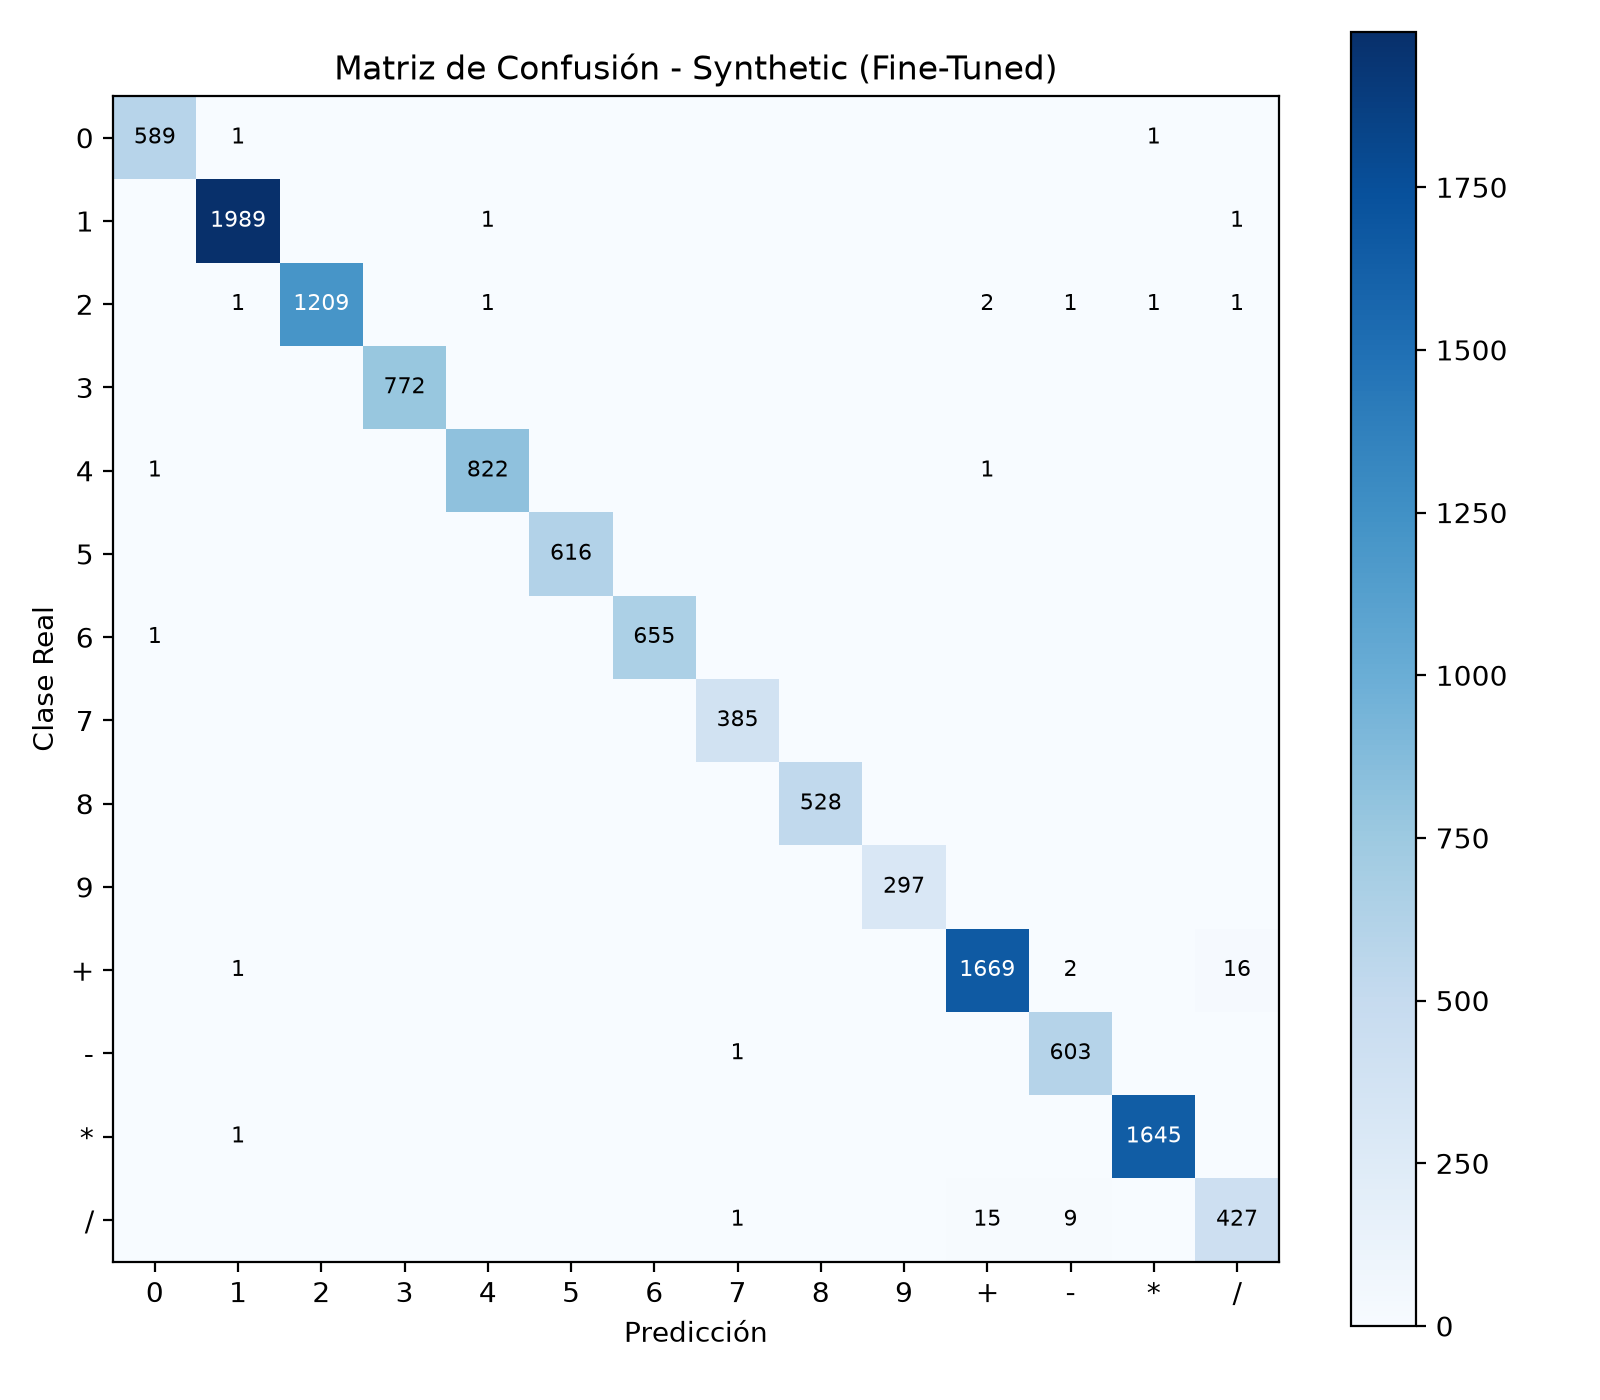
\includegraphics[width=0.88\linewidth]{figs/ocr_finetuned_synthetic_confusion.png}
\caption{Matriz de confusi\'on de \texttt{GlyphCNN} en el dataset Synthetic Normal ($12{,}266$ glifos clasificados).}
\label{fig:conf_normal}
\end{figure}

\begin{figure}[htbp]
\centering
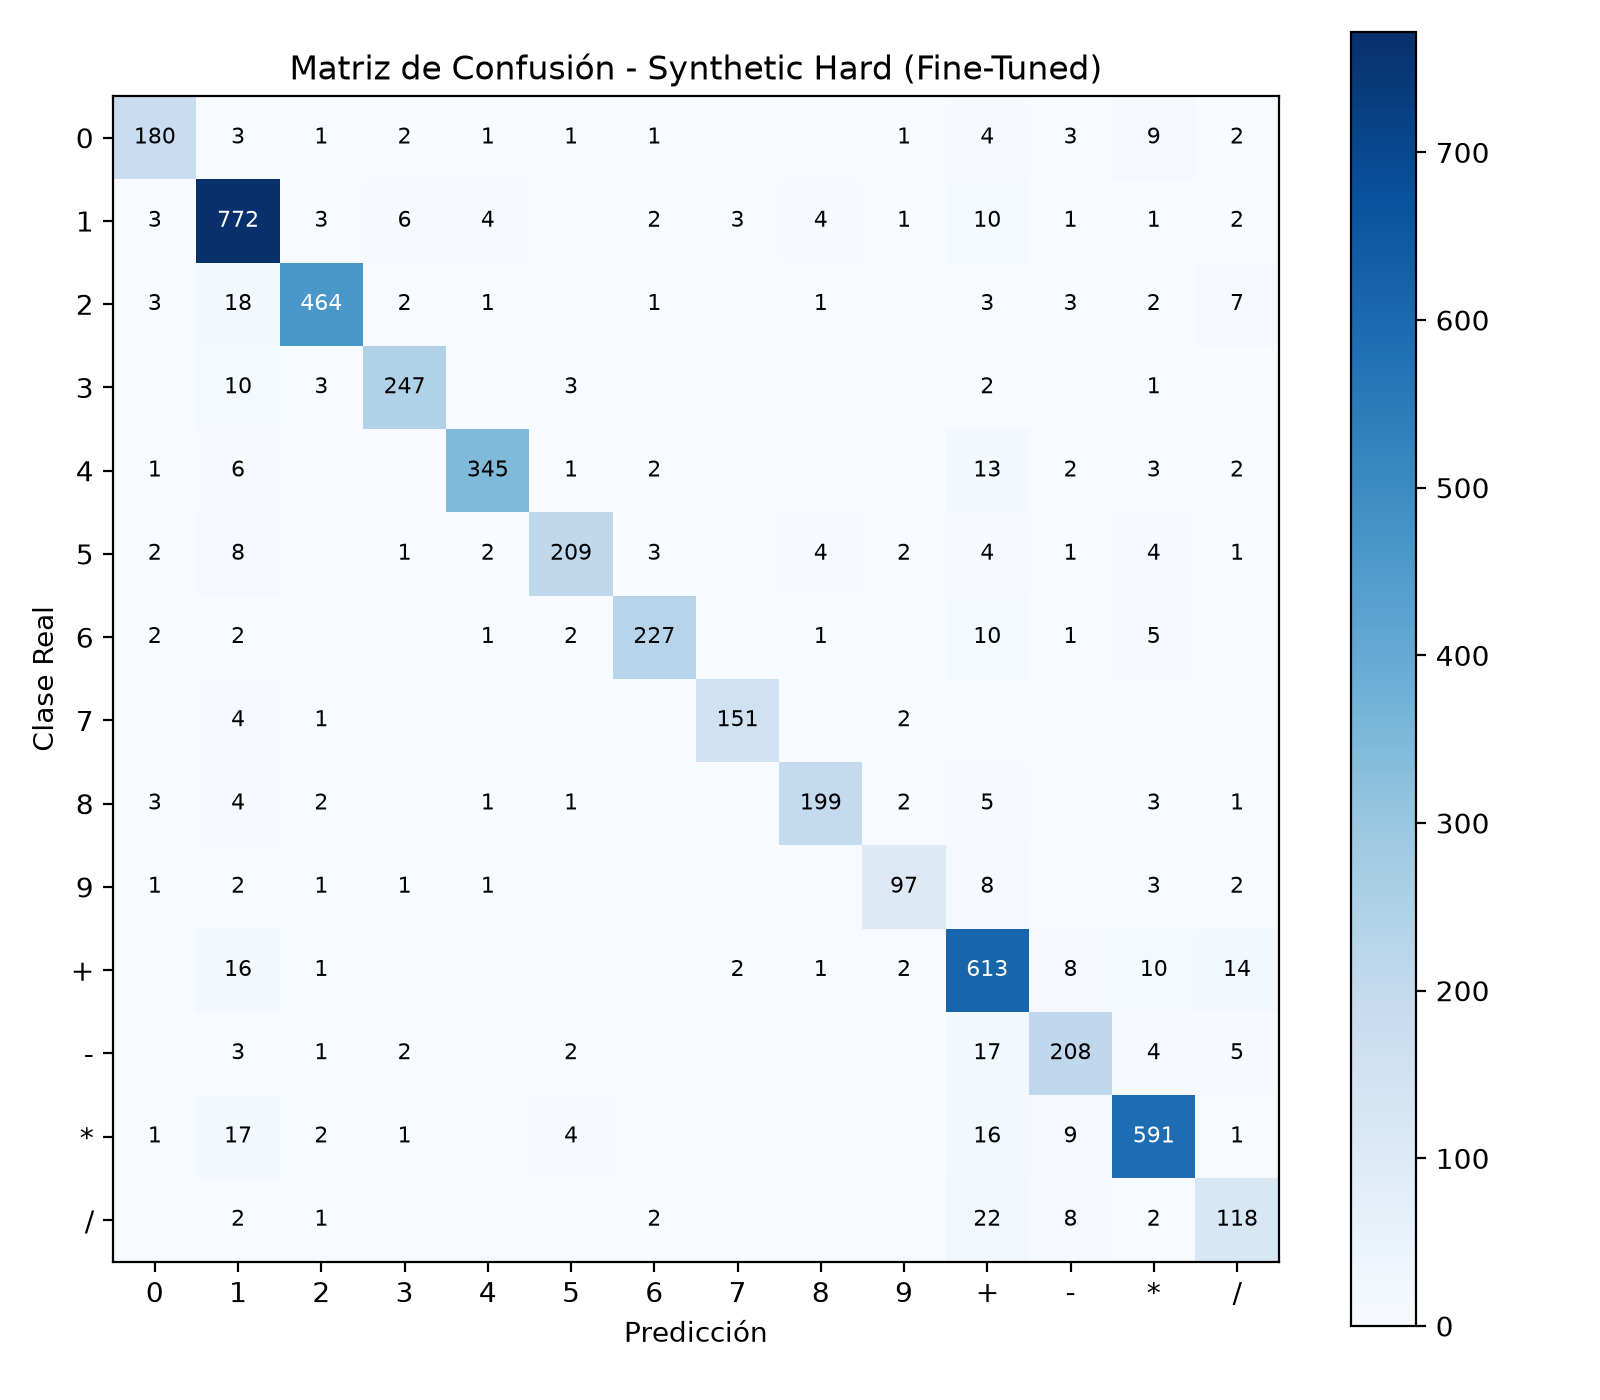
\includegraphics[width=0.88\linewidth]{figs/ocr_finetuned_hard_confusion.png}
\caption{Matriz de confusi\'on de \texttt{GlyphCNN} en el dataset Synthetic Hard ($4{,}859$ glifos con ruido y sombras severas).}
\label{fig:conf_hard}
\end{figure}

\begin{table}[htbp]
\caption{Desempe\~no por Clase: F1-Score (\%) a Trav\'es de los Datasets}
\label{tab:char_f1}
\centering
\footnotesize
\setlength{\tabcolsep}{3.2pt}
\begin{tabular}{@{}ccccc@{}}
\toprule
\textbf{Glifo} & \textbf{F1 Normal} & \textbf{F1 Hard} & \textbf{F1 Stress} & \textbf{Vulnerabilidad} \\
\midrule
$\div$ & 95.21\% & \textbf{76.13\%} & \textbf{70.87\%} & \textbf{Cr\'{\i}tica} \\
$-$    & 98.93\% & 85.60\% & 85.29\% & Alta \\
$+$    & 98.90\% & 87.95\% & 91.24\% & Moderada \\
$\times$& 99.91\% & 92.34\% & 98.55\% & Baja \\
$0$    & 99.66\% & 89.11\% & 94.17\% & Moderada \\
$1$    & 99.85\% & 91.96\% & 95.58\% & Baja \\
$2$    & 99.71\% & 94.21\% & 97.14\% & Baja \\
$3$    & 100.00\% & 93.56\% & 93.72\% & Baja \\
$4$    & 99.76\% & 94.39\% & 98.35\% & Baja \\
$5$    & 100.00\% & 90.09\% & 97.65\% & Moderada \\
$6$    & 99.92\% & 92.84\% & 96.12\% & Baja \\
$7$    & 99.74\% & 96.18\% & 96.70\% & Baja \\
$8$    & 100.00\% & 92.34\% & 98.01\% & Baja \\
$9$    & 100.00\% & 87.00\% & 97.50\% & Moderada \\
\bottomrule
\end{tabular}
\end{table}

Las cinco confusiones f\'{\i}sicas m\'as recurrentes observadas fueron:
\begin{enumerate}
    \item $\div \to +$ (52 casos): La barra oblicua $\div$ al intersectar remanentes de cuadr\'{\i}cula genera un pseudotrazo horizontal que activa los filtros de $+$.
    \item $+ \to \div$ (40 casos): Degradaci\'on lum\'{\i}nica aten\'ua un brazo de $+$, simulando una l\'{\i}nea diagonal ante \'angulos leves de inclinaci\'on.
    \item $- \to +$ (26 casos): Remanentes verticales de la celda que contactan el centro del guion transforman la l\'{\i}nea en cruz.
    \item $2 \to 1$ (24 casos): En celdas de alta densidad ($8\times8$, $9\times9$), los arcos del d\'{\i}gito $2$ pierden contraste, reteniendo \'unicamente el trazo vertical.
    \item $\times \to +$ (18 casos): El glifo de multiplicaci\'on difiere de $+$ \'unicamente por rotaci\'on de $45^\circ$, solapando filtros ante rotaci\'on residual.
\end{enumerate}
